% THIS IS A LATEX TEMPLATE FILE FOR PAPERS INCLUDED IN THE
% *Anthology of Computers and the Humanities*. ADD THE OPTION
% 'final' WHEN CREATING THE FINAL VERSION OF THE PAPER. 
% DO NOT change the documentclass
\documentclass[final]{anthology-ch} % for the final version
%\documentclass{anthology-ch}         % for the submission

% LOAD LaTeX PACKAGES
\usepackage{booktabs}
\usepackage{graphicx}
\usepackage{subcaption}
% ADD your own packages using \usepackage{}
\usepackage{hyperref}

\usepackage{xcolor}
\usepackage{colortbl}
\usepackage{array}     
\usepackage{tikz}

\newcommand{\theo}[1]{{\textcolor{blue}{#1}}}


% TITLE OF THE SUBMISSION
% Change this to the name of your submission
\title{Transmission and Survival of Iberian Patristic Texts (3rd–5th Centuries)}


% AUTHOR AND AFFILIATION INFORMATION
% For each author, include a new call to the \author command, with
% the numbers in brackets indicating the associated affiliations 
% (next section) and ORCID-ID for each author.  
\author[1]{Émilie Guidi}[
  orcid=0009-0009-1852-2070
]

\author[1]{Théo Moins}[
  orcid=0009-0002-7191-5761
]

% While we encourage including ORCID-IDs for all authors, you can
% include authors that do not have one by definining an empty ID.

\author[1]{Jean-Baptiste Camps}[
  orcid=0000-0003-0385-7037
]

% There should be one call to \affiliation for each affiliation of
% the authors. Multiple affiliations can be given to each author
% and an affiliation can be given to multiple authors. 
\affiliation{1}{École nationale des chartes, Université PSL, Paris, France}

% KEYWORDS
% Provide one or more keywords or key phrases seperated by commas
% using the following command
\keywords{Unseen Species, Agent-Based Modelling, Birth-and-Death Process, Cultural Transmission, Philology, Patristics}

% METADATA FOR THE PUBLICATION
% This will be filled in when the document is published; the values can
% be kept as their defaults when the file is submitted
\pubyear{2025}
\pubvolume{3}
\pagestart{556}
\pageend{574}
\conferencename{Computational Humanities Research 2025}
\conferenceeditors{Taylor Arnold, Margherita Fantoli, and Ruben Ros}
\doi{10.63744/WVZDLY7xI2fT}  
\paperorder{35}

\addbibresource{bibliography.bib}

%RAPPEL DU CALL%
% short papers: up to 3000 words (ca. 6 pages, references, abstract and tables/illustrations excluded).

\hyphenation{ma-nu-scripts}

%%%%%%%%%%%%%%%%%%%%%%%%%%%%%%%%%%%%%%%%%%%%%%%%%%%%%%%%%%%%%%%%%%%%%%%%%%%
% HERE IS THE START OF THE TEXT
\begin{document}

\maketitle

\begin{abstract}
%This paper presents an analysis of the textual transmission of the Church Fathers from the Iberian Peninsula using computational methods. The corpus, limited to this geographic area, includes patristic texts characterised by formal diversity (prose, verse) and generic variety (sermons, letters, chronicles, epics). Exploring this heterogeneity highlights two antagonistic transmission dynamics: prose texts have a higher richness but are transmitted with fewer witnesses, often maybe only thanks to their inclusion in medieval collections. On the other hand, poetic texts, fewer in number but part of large literary projects, have generated a high number of witnesses. These formal and material specificities are then linked to models of textual transmission. Two recent approaches were explored: probabilistic modelling using unseen species models, which provided a first estimation of the survival and loss rates of texts and their witnesses and revealed a corpus with low diversity and evenness scores; and stochastic modelling, more focused on cultural evolutionary dynamics, aimed at analysing the evolution of witness populations through a birth-death model. 
%Results hint at a survival rate of texts below 67\% and perhaps closer to 20\%, and a survival rate of manuscript below 10\%, and perhaps below 1\%. 
%Interestingly, even though previous research had shown that unseen species and birth-death processes could yield similar estimates in terms of survival of texts for Medieval French literature, here the figures obtained are substantially different, pointing to the potential effects of diachrony, in terms of chronological range, in the provided results. 
%The results also confirm some inadequacies of a simple birth-death process to fully account for some of the dynamics of text transmission, related in particular to very successful texts and to variation in time of production and destruction rates.
This paper analyses the textual transmission of the Church Fathers from the Iberian Peninsula. The corpus is characterised by formal (prose, verse) and generic (sermons, letters, chronicles, epics) heterogeneity. Our computational analyses reveal two contrasting transmission dynamics: prose texts are more numerous but are transmitted by fewer witnesses, sometimes only via their inclusion in medieval collections. Poetic texts, fewer in number, have generated a higher number of witnesses, likely due to their integration in large literary projects.

We model these dynamics using two approaches: \textbf{probabilistic unseen species models}, which estimate an upper bound of text and witness survival rates and indicate low corpus diversity and evenness; and \textbf{stochastic birth-death models}, which explore cultural evolutionary patterns in text and witness populations. Results suggest a text survival rate below 67\% (potentially closer to 20\%) and a manuscript survival rate below 10\% (possibly under 1\%).

Notably, these estimates diverge from prior findings for Medieval French literature, where unseen species and birth-death models yielded similar results. This discrepancy suggests that diachrony --\,specifically, the broader chronological range of the patristic corpus\,-- plays a key role in shaping transmission outcomes. Our findings also highlight limitations of the birth-death model, particularly in accounting for highly successful texts and in temporal variations in production/destruction rates.
\end{abstract}

\section{Introduction} 

\subsection{Computational methods for textual transmisssion}

% Why is this corpus important? What are its historical specificities?
% Why is it interesting to study it, and for what goals?
% RESEARCH QUESTION
% STATE OF THE ART
% Why was this method chosen ? These methods (if time)? Why is it useful to compare them?

%Our understanding of human culture is based, among other things, on material artefacts. In the field of textual history, much of this knowledge is embodied in manuscripts. However, manuscripts should not be seen as isolated objects of study, but as links in a wider chain of textual transmission.
In the field of textual history, textual transmission designates the way a text is disseminated and preserved through the copy of material artefacts like manuscripts.
This process of transmission is neither linear nor static; it follows an evolutionary dynamic marked by processes of dissemination, selection, variation and extinction. 
Books are first produced --\,for instance, in the case of patristic texts we envision here, manuscripts are usually copied in scriptorial workshops linked to libraries or monastic schools, where scribes copy them with a view to preserving them~\cite{Bischoff}.
Their diffusion, whether immediate or spread over the long term, depends on a number of factors, in particular the decision to reproduce certain texts rather than others. Liturgical manuscripts and the major texts of the Fathers of the Church were widely copied. Texts from Classical and Late Antiquity were also favoured, as they were often used in schools to teach reading and rhetoric. Some manuscripts disappeared, whether for human or natural reasons (gradual loss of interest in a work, library fires, wars, etc.), while others were reused, prolonging their existence in new contexts. The manuscript tradition thus reflects different uses and intentions at different times. It evolves, transforms and adapts according to chance and to the needs and views that societies have of texts.  

Traditional manuscript sciences have long been the principal tools used to describe a textual tradition. Palaeography focuses on the evolution of scripts, while codicology focuses on the material aspects of manuscripts. Philology, which notably includes ecdotics and textual criticism, concentrates on the linguistic and literary study of texts, sometimes attempting to reconstruct earlier versions, or even lost versions, of them \cite{muzerelle}. In particular, textual criticism aims to examine the variants present in the different witnesses, organise them in a genealogical perspective, and restore the earliest accessible form of a text based on the available evidence. While these disciplines can help to recover certain aspects of a lost manuscript tradition, they are nevertheless unable to grasp the tradition in its entirety.

This is precisely where new approaches come into play, made possible by the development of computational humanities. Recent years have seen the emergence of  computational methods applied to the study of textual transmission, with the aim of modelling the dynamics of loss and survival. Two main approaches have emerged. The first, developed as part of the \textit{Forgotten Books} project~\cite{kestemont}, applies models of unseen species derived from ecology to manuscript traditions, from a probabilistic perspective. The second, carried out by the \textit{ERC-LostMA} project~\cite{camps2025transmissiontextswrittencultures}, uses stochastic processes of the birth-and-death type, coupled with computer simulations, in the direction pioneered by the work of Weitzman~\cite{weitzman_1987} and Cisne~\cite{cisne}.

\subsection{Contributions}

The main objective of our work is to apply these recent approaches to patristic texts produced in the Iberian Peninsula between the mid-3rd century and the mid-5th century.
This textual tradition is still unexplored with such methods, which has so far concentrated on ancient texts~\cite{weitzman_1987}, medieval scientific manuscripts~\cite{cisne}, or chivalric narratives~\cite{kestemont}.
Studying the transmission of a corpus in this pivotal period between Classical Antiquity and the Middle Ages from this perspective remains therefore unprecedented. %This longer duration than that observed for medieval corpora invites us to question potential differences in loss rates between ancient and medieval texts.
We can wonder whether this corpus follows similar patterns of transmission and loss than those previously studied, or if the difference in the length of the period envisioned, and the mode of transmission and reception of those texts (particularly confronted with vernacular fictional literature studied in previous projects) will be revealed through computational analysis. 


This study aims to model the transmission of the patristic tradition in the Iberian Peninsula by estimating the survival and disappearance rates of texts and manuscript witnesses. It also examines whether distinct dynamics emerge in the processes of conservation, diffusion, and extinction depending on textual form, particularly between prose and poetry. For this purpose, we will employ probabilistic models, especially those of unseen species~\cite{kestemont}, as well as stochastic processes~\cite{camps2025transmissiontextswrittencultures}.
The approach relies on the creation of a new database recording all known manuscript sources of the Iberian patristic tradition of texts originating between the 3rd and the 5th century. It also proposes the application, for the first time, of computational methods to this corpus, which involves adapting the existing computational models to the specific features of Late Antiquity, in order to better account for the dynamics specific to this period.


% Contributions 

\section{Material}

\subsection{Data collection}

The constitution of the corpus involved manual data collection, consisting of an inventory of the texts of the Church Fathers active in the Iberian Peninsula between the 3\textsuperscript{rd} and 5\textsuperscript{th} centuries, as well as the identifiable manuscript witnesses that transmitted them. The selection focused exclusively on the direct tradition, including both preserved manuscripts (complete or fragmentary) and those whose existence is attested despite their loss (fire, war, etc.), but not the derived works. %EXEMPLE?
This corpus covers the geographical area of the Iberian Peninsula, corresponding to the territories of present-day Spain and Portugal. This choice is particularly relevant because the tradition from this period is well documented and has recently been the subject of critical editions \cite[see][]{TradPat}.


It is delimited chronologically by the Councils of Nicaea (325) and Chalcedon (451), in accordance with the boundaries established by the \textit{Clavis Patrum Latinorum}~\cite{Dekkers1995}. Authors of Late Antiquity (6\textsuperscript{th}-7\textsuperscript{th} centuries) have been deliberately excluded, since many of their texts have not yet been reliably edited or their manuscript tradition studied in depth.
The identification of texts and authors was done mainly on the basis of the \textit{Clavis Patrum Latinorum}~\cite{Dekkers1995} {[henceforth \textit{CPL}]},  supplemented by the \textit{Traditio Patrum, Scriptores Hispaniae}~\cite{TradPat}. Authors were selected who were either of Iberian origin or who were active in the region. Texts attributed with certainty, but also those described as \textit{dubia} or \textit{spuria}\footnote{Works considered \textit{dubia} are those whose attribution is questioned, and works considered \textit{spuria} are those whose attribution has been recognised as false.}, were included,  as long as their author's origin was recognised as Iberian. Two anonymous texts have also been included (\textit{CPL}, 789 and 373a), their production context being located on the Iberian peninsula.

Indirect tradition has been deliberately excluded from our study. In our corpus, it manifests itself in a variety of forms. Some texts are taken up, summarised or adapted in other works. This is particularly true of the \textit{Chronicle} of Hydace, an epitome of which is incorporated into later compositions such as the \textit{Historia Gothorum, Wandalorum et Suevorum} (\textit{CPL} 1204) by Isidore of Seville, or the \textit{Pseudo-Fredegarius}. This phenomenon also applies to poetry, where texts such as those by Prudentius served as models or were taken up in intertextual chains, notably involving Arator's \textit{Apostolic History}, Corippus' \textit{Johannides} or, more recently, Milon de Saint-Amand's \textit{De Sobrietate}.
A second case that is also excluded is that of recensions, as shown by the example of Montanus of Toledo, whose \textit{Epistulae} (\textit{CPL}, 1094) circulated within the \textit{Collectio Hispana}. The latter itself gave rise to derivative versions, such as the \textit{Hispana Gallica}.

%Texts both in prose and in versified form were retained, which results in a certain generic heterogeneity. 
Excluding indirect tradition and recensions thus allows us to focus on the corpus proper and the diversity of its textual forms, both in prose and versified form.
On the prose side, we find a wide variety of genres: letters and treatises, writings related to preaching such as sermons and homilies, texts of confession of faith such as \textit{credo}, foundational texts such as ecclesiastical canons, as well as historiographical texts including historical chronicles. 
It is worth highlighting a specific feature of the transmission of the texts in our corpus: Late Antique texts circulated in the form of collections~\cite{gioannicollection}, structured according to thematic or generic coherence. Some texts owe their preservation to their inclusion in homilies, others to their inclusion in canonical collections. Still others have been preserved as part of vast doctrinally-oriented collections, notably on themes such as Priscillianism and other theological controversies. The Ancients did very little theorising on literary genres, a fact that is particularly evident in prose, which contains many hybrid work, such as the ``lettres-traités'', that blend correspondence and morale treatise.
The text \textit{De similitudine carnis peccati} (\textit{CPL}, 567) by the priest Eutrope is a representative example as it's a letter addressed to Caesaria, a pious woman, combining the personal form of an epistolary exchange with a structured theological argument on the nature of Christ and the incarnation.  
On the poetic side, the corpus includes verse texts ranging from relatively short poems covering a variety of themes such as panegyric, lyrical, satiric, and didactic pieces, to large-scale works such as epics, which are represented by major figures like Prudentius and Juvencus.



\subsection{Corpus analysis}

Applying these criteria, we assembled a corpus of $M = 1159$ manuscripts corresponding to $T = 67$ texts by 37 different authors. 
The oldest manuscripts date from the 6th century, while we set the 15th century as the upper limit, since in our tradition manuscripts later than the 15th century are often copies based on printed editions, whereas we are primarily interested in witnesses of the manuscript tradition itself. 
Their provenance spans the whole of Europe.


\begin{figure}
    \centering
    \begin{subfigure}[c]{0.55\textwidth}
        \centering
        \includegraphics[width=\textwidth]{figures/witness_dist.png}
        \caption{Abundance data distribution for prose and poetry.}
        \label{fig:pvsp_dist}
    \end{subfigure}
    \hfill
    \begin{subfigure}[c]{0.35\textwidth}
        \centering
        \begin{tabular}{lcccc}
            \toprule
            \textbf{Genre} & \textbf{$f_1$} & \textbf{$f_2$} & \textbf{$T$} & \textbf{$M$} \\
            \midrule
            Poetry & 3  & 1 & 6  & 365 \\
            Prose  & 16 & 4 & 61 & 794 \\
            Total & 19 & 5 & 67 & 1159 \\
            \bottomrule
        \end{tabular}
        \caption{Singletons $f_1$, doubletons $f_2$, number of texts $T$ and number of manuscript witnesses $M$ for each part of the corpus.}
        \label{tab:abundance_genre}
    \end{subfigure}
    \begin{subfigure}[c]{0.6\textwidth}
        \includegraphics[width=\textwidth]{figures/evennesspvsp.png}
        \caption{Evenness profiles for prose and poetry texts across orders \textit{q}}
        \label{fig:evennesspvsp}
    \end{subfigure}
    \caption{Abundance and evenness comparison for prose and poetic texts.}
    \label{fig:pvsp}
\end{figure}

The dataset is illustrated in~\autoref{fig:pvsp}, and highlights a marked contrast between the two genres. 
Prose exhibits a significantly greater richness, with 61 distinct texts identified, compared to only 6 for poetry. 
However, despite this disparity in textual diversity, poetry shows a remarkably high total abundance ($M = 365$ poetry manuscripts), concentrated in a small number of works. 
In contrast, the 61 prose texts collectively amount to a total abundance of $M = 794$, see~\autoref{tab:abundance_genre}. 
This disproportionate distribution indicates a strong transmission dynamic for a small number of poetic texts, reflecting their cultural or literary prominence in our corpus.
To further characterize this distribution, we plot in~\autoref{fig:evennesspvsp} diversity profiles based on the parameter \( q \), which controls the sensitivity to dominant versus rare elements: at \( q = 0 \), diversity corresponds to richness (number of distinct texts), while higher values of \( q \) progressively emphasize the most abundant texts. 
Evenness, derived from these profiles, measures how equitably transmission is distributed across texts, with values near 1 indicating balanced distribution and lower values reflecting concentration around a few dominant works.
As shown in \autoref{fig:evennesspvsp}, the evenness profiles reveal a marked difference between prose and poetry texts. 
Across all orders \( q \), the curve corresponding to poetry declines more rapidly and reaches significantly lower values than that of prose. 
This steep drop, observable even at low values of \( q \), indicates a strong concentration of transmission around a few highly dominant poetic works, to the detriment of the rest of the corpus. 
In contrast, the prose curve follows a more gradual slope and maintains higher evenness values, suggesting a more balanced distribution among the various texts.
How can we explain and model the fact that poetic texts, though fewer in number, were widely transmitted and frequently copied?
In particular, how does this specific behaviour influence our analyses of text survival?
A first response would be to make two separate studies for poetry and prose, but the small number of poetry samples forces us for now to study only the prose texts for the rest of the study.
Results on the entire corpus (prose and poetry) are also given and discussed in \autoref{app:full_patristic-corpus}.


\section{Methods}

\subsection{Unseen Species Model}

Recent research demonstrated that the statistical diversity estimators, traditionally commonly used -~among other fields~- in ecology, can also be successfully applied to cultural heritage~\cite{kestemont}.
The non-parametric methods, such as unseen species models, make it possible to estimate total richness (i.e., the total number of species, or texts in our case) and diversity of a population, by integrating unobserved elements, and correct the bias induced by the frequent presence of rare species, a major characteristic of our corpus. In particular, the \textit{Forgotten Book} project applied several estimators to a corpus of European medieval chivalric narratives, in several languages, thanks to which the authors were able to estimate a minimal number of unseen (i.e. lost) texts and manuscript witnesses~\cite{kestemont}. The methods they introduced to the field of philology were made available in the \textit{Copia} Python package, that has also since been enriched with additional estimators \cite{kestemont2025copia}.

We choose three estimators used in \textit{Forgotten Books}~\cite{kestemont}: Chao1 \cite{chao1984nonparametric}, iChao1 \cite{chiu2014} and Jackknife \cite{burnham1978estimation}. The Chao1 estimator provides a minimum bound on the original richness based on texts preserved in one or two witnesses (singletons and doubletons), while iChao1 refines this estimate by also including texts present three or four times, thus reducing the risk of underestimation. 
This approach is particularly well-suited to our corpus, in which 40\% of the texts (27 in total) are transmitted by only a very small number of witnesses (one to four witnesses). 
The Jackknife estimator stands out for its ability to take into account the heterogeneity of the distribution of texts, which is crucial in a corpus where a small number of widely distributed texts, such as Prudentius texts that total almost 300 witnesses, coexist with others that are extremely rare. 
Unlike Chao1 and iChao1, which rely mainly on the frequency of the rarest texts, Jackknife uses a systematic resampling mechanism that exploits all the frequencies of appearance, providing a nuanced estimate of the original richness\footnote{%
    Although the ACE estimator is available in the Copia package~\cite{kestemont2025copia}, we do not consider this method here as it requires an arbitrary abundance threshold corresponding to the upper limit for considering a species as rare, and complicates comparison between estimations made on different corpora, that could require the use of different thresholds.
    Similarly, Egghe's estimator~\cite{egghe2007estimation}, also implemented in Copia but initially designed for printed corpora with a known number of print runs, is not relevant to a manuscript tradition.
}.
%By default, this threshold follows recommendations from the ecological EstimateR package \theo{add citation}, where species observed 10 times or fewer are typically classified as rare. 
%While this parameter can technically be lowered, it remains difficult to determine what should count as a rare text in our corpus. 
%The concept of rarity is less clearly defined in textual datasets than in ecological ones, and the choice of such a threshold is not easily justifiable. % For these reasons, the ACE estimator was not only excluded from our analysis, but was also not employed in the prior application to vernacular chivalric narratives~\cite{kestemont}.

In order to estimate the minimum number of witnesses that would need to be observed in order to register all the unobserved texts in the Iberian patristic tradition, we used the estimator \textit{Minimum Additional Sampling}~\cite{kestemont}, included in \textit{Copia}, that was used to estimate the survival rates for documents preserving romances and heroic narratives in different linguistic traditions~\cite{kestemont}. This estimator allows us to estimate how many additional witnesses would be required for an extended sample to contain at least one occurrence of each original text. It is based on the dynamics of singletons when the sample is enlarged: those already present in the initial sample versus those newly discovered. 

 %The appearance of an asymptotic plateau indicates that the majority of original texts have been identified. The combined use of the MAS estimator and this curve makes it possible to evaluate the rate of documentary loss and to estimate the potential still to be discovered

On the basis of these richness estimators, we also estimated the survival rate of texts and witnesses: to do this, we converted the estimates of textual and witness richness into survival proportions, by relating the estimated richness to the richness actually observed. 
We then generated density curves by resampling using the \textit{bootstrap} method, making it possible to visualise the variability of the survival rates for each estimator selected (see below, \autoref{fig:richesse_et_survie} and \autoref{fig:images_cote_a_cote}). 
%Finally, we assessed the internal diversity of the corpus by plotting an evenness profile. % based on the order of diversity (below, \autoref{fig:evenness} and \autoref{fig:hill}). 
%Whereas simple specific richness counts only the number of distinct texts, Hill numbers integrate both richness and relative abundance, modulating sensitivity to frequent texts. This family of indices offers a more detailed view of the structure of textual diversity. At the same time, 
%The normalised evenness measure provides information about the homogeneity of the distribution of abundance: high evenness indicates a balanced distribution of texts, while low evenness reveals the dominance of a small number of texts in manuscript transmission (\autoref{fig:evennesspvsp}).
%\theo{Ce dernier paragraphe c'est déjà un peu des résultats peut être, surtout si l'on se référence aux figures?}

% plus robuste quand taille échantillon plus petite: si ordre élevé pas 

% Indicateurs choisis, leur pertinence (Chao, iChao, Jacknife? + Min_sample? ou approche alternative?)
% Rappel des méthodes envisagées

\subsection{Modelling the dynamics of text transmission}

Alternatively, one can consider a dynamic approach by simulating the temporal evolution of both text and witness populations, in order to reconstruct the evolutionary processes that led to the formation of our current corpus.
The real-world dynamics of transmission or extinction of texts were probably influenced by a multiplicity of factors, be they extrinsic (fires, wars, economic crises, etc.) or intrinsic (different fitness of the texts or the witnesses, reception and reader interest, etc.). %Yet, in order to model this process, it can be reduced to a set of core elements, chosen to reflect the core transmission dynamics. 
From the modelling perspective, the core transmission dynamic reduces to a new text appearing with an original witness (the authorial manuscript), and witnesses that can be copied and/or destroyed in time. %This dynamic results from multiple factors, both natural (fires, wars, degradation) and human (changing interest, copying success). By reducing transmission to its essentials, each new text appear with an original witness (the authorial manuscript); witnesses can be copied and/or destroyed in time. 
For each text, this implies two outcomes: survival if there is more copy than destruction, or disappearance.
% This dynamic of preservation and extinction may result from multiple factors, both natural (fires, wars, material degradation) and human (gradual loss of interest in a work, or conversely, success leading to widespread dissemination through copying).
% Thus, by reducing textual transmission to its essential components, we can conceptualize each manuscript as belonging to a population that evolves according to two possible outcomes: either its documents are more copied than destroyed and thus the texts survives (including in derived or innovated forms), or it disappears.

A primary method for modelling involves employing a birth-death process with constant rates~\cite{weitzman_1987, camps2025transmissiontextswrittencultures}: each witness is modelled as an independent agent, from which copies are made with rate $\lambda$ per unit time and that can be destroyed with rate $\mu$.
A recent update applied to Medieval chivalric literature~\cite{camps2025transmissiontextswrittencultures} allows parameters $\lambda$ and $\mu$ to be estimated from observations, in a model with a temporal division into two distinct phases: a period of activity, when texts were actively transmitted and copied in manuscript form, and a period of inactivity when the texts are no longer copied, but witnesses can still be destroyed, and so $\lambda$ is fixed at 0 but not $\mu$ (modelling the period after the appearance of the printing press). 
Obtaining an estimate of $\lambda$ and $\mu$ allows to deduce an estimate of quantities of interest such as survival rate, extinction probability, topological properties of trees, etc., either by mathematical derivation or by re-simulations of this process with estimated parameters.

Yet, our corpus presents a relatively different type of tradition, particularly regarding chronological parameters, since the texts go back to Late Antiquity. 
Moreover, while the texts were conceived by authors from the Iberian peninsula, during a limited amount of time (the 3rd to 5th centuries), copies continued to be actively produced throughout Europe during the centuries of the Middle Ages.
Therefore, some adaptations are needed with respect to the model used by Camps et al.~\cite{camps2025transmissiontextswrittencultures}, in order to distinguish a period of both texts and witnesses creation, to a period where no new text appear but witnesses keep being reproduced.
%First, the focus of this birth-death process is mainly on the dynamics of witnesses , and not the dynamics of texts. 
%Although we can calculate the survival rate of a tree from the dynamic of its nodes, and the death of a tree results in the death of all its surviving manuscripts, the question of the birth of a new text should be included in the model.
%A second major difference between this corpus of patristics texts and the medieval narratives in \cite{camps2025transmissiontextswrittencultures} is the decorrelation between the production of texts and the production of manuscripts. 
%During Late Antiquity, texts were indeed produced, but during the Middle Ages, they were only transmitted. 
%The model does not allow us to distinguish this period of text creation from one of simple transmission.

% Description d'une simulation
To overcome these obstacles, we suggest a model of transmission divided into three phases:
\begin{enumerate}
    \item \textbf{An innovation phase (201–500)}:
    This corresponds to Late Antiquity, when patristic authors were actively producing new texts while existing texts were simultaneously being transmitted through manuscript copying.
    During this period, new independent texts are created while existing manuscript witnesses continue to be copied and potentially destroyed. 
    This phase is characterized by the two parameter $\lambda$ (copying rate) and $\mu$ (destruction rate), but also by a third one, $\Lambda$, for new tree creation per unit time.
    $\Lambda$ act as an innovation rate, and is not proportional to the average population (contrary to $\lambda$ and $\mu$), but represents the external appearance of a new text.
    
    \item \textbf{A reproduction phase (501–1450)}:
    This corresponds to the medieval period, when patristic texts were no longer being authored but were actively transmitted throughout Europe through manuscript copying, with scribes reproducing existing texts without creating fundamentally new texts.
    This phase is marked by the cessation of new text creation ($\Lambda = 0$), while existing witnesses continue to be copied and destroyed according to rates $\lambda$ and $\mu$ respectively. 
    
    \item \textbf{An inactive phase (1451–1700)}:
    This phase typically corresponds to the post-medieval period, particularly after the advent of printing, when manuscript copying was largely abandoned while existing witnesses remained vulnerable to loss and destruction.
    During this final period, copying activity ceases ($\lambda = 0$), leaving only the destruction rate $\mu$ active. 
    Witnesses can still be lost through various factors (wars, fires, material degradation, neglect) but are no longer being reproduced. 
\end{enumerate}

\begin{figure}[htbp]
    \centering
    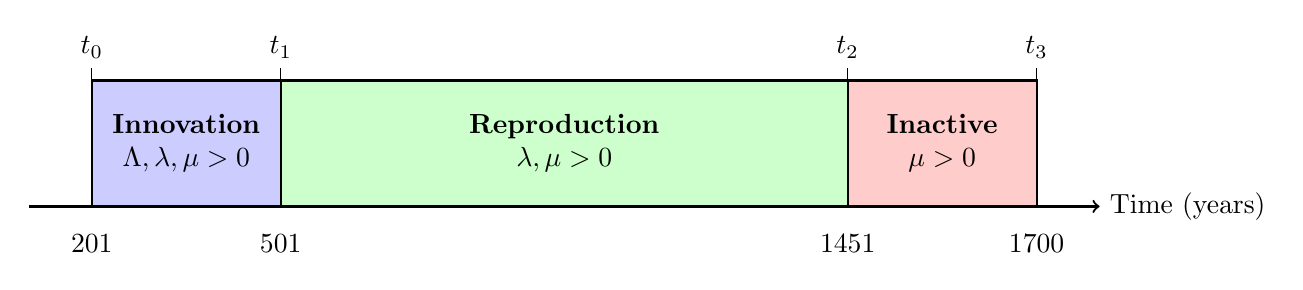
\begin{tikzpicture}[scale=0.8]
        % Timeline
        \draw[thick, ->] (-1,0) -- (16,0) node[right] {Time (years)};
        
        % Time points
        \draw (0,1) -- (0,2.2) node[above] {$t_0$};
        \draw (3,1) -- (3,2.2) node[above] {$t_1$};
        \draw (12,1) -- (12,2.2) node[above] {$t_2$};
        \draw (15,1) -- (15,2.2) node[above] {$t_3$};
        
        % Year labels
        \node[below] at (0,-0.3) {201};
        \node[below] at (3,-0.3) {501};
        \node[below] at (12,-0.3) {1451};
        \node[below] at (15,-0.3) {1700};
        
        % Phase bars
        \draw[fill=blue!20, thick] (0,0) rectangle (3,2);
        \draw[fill=green!20, thick] (3,0) rectangle (12,2);
        \draw[fill=red!20, thick] (12,0) rectangle (15,2);
        
        % Phase labels
        \node[align=center] at (1.5,1) {\textbf{Innovation} \\ $\Lambda, \lambda, \mu > 0$};
        \node[align=center] at (7.5,1) {\textbf{Reproduction} \\ $\lambda, \mu > 0$};
        \node[align=center] at (13.5,1) {\textbf{Inactive} \\ $\mu > 0$};
        
        
    \end{tikzpicture}
    \caption{Timeline of the three-phase transmission model with active parameters for each period.}
    \label{fig:timeline}
\end{figure}

% Description du modèle mathématique

A diagram of the different periods, along with the definition of the time points $t_i$'s, that mark the start/end times for each phase, is summarised in \autoref{fig:timeline}.
This model allows an explicit calculation of quantities of interest like the richness or the proportion of surviving texts and witnesses at $t_3$, as a function of the parameters $(\Lambda, \lambda, \mu)$ and duration of the different phases $t_i$. 
The various formulas are given in \autoref{sec: app_maths}.

% Inference methodology

Parameter estimation for $(\Lambda, \lambda, \mu)$ from observed data constitutes a classical inverse problem: while we can simulate this kind of process from given parameters, we need to infer parameters from observed data.
We employ here Simulation-Based Inference (SBI)~\cite{cranmer2020frontier}, which simulates the transmission process across various parameter combinations and learns the mapping between parameters and resulting data to identify the most probable parameters generating our observations.
Unlike point estimation methods, this Bayesian framework provides full posterior probability densities $p(\Lambda, \lambda, \mu \mid \text{data})$, quantifying uncertainty in parameter estimates and enabling robust statistical inference.
Therefore, all the quantities of interest obtained by parameter transformation such as richness will be probabilistic, and so all density of probability will be available for inference, in particular to describe the uncertainty around the estimation (more details in \autoref{sec:prior}).
The method requires defining a prior distribution $p(\Lambda, \lambda, \mu)$ over parameter space: we use constrained uniform priors that enforce biological constraints (e.g., $\lambda > \mu$ for population growth) and computational limits through a maximum population threshold \texttt{max\_pop} to prevent memory overflow during simulation. 
%This approach simulates the transmission process at discrete time steps (quarterly periods) and compares summary statistics from simulated data with those from observed manuscript counts.
The inference pipeline, implemented in the \texttt{simmatree} package~\cite{moins_2025_17425020}, uses Neural Posterior Estimation~\cite{NPE} to approximate the posterior distribution directly via neural networks.\footnote{%
    The package also offers multi-round refinement to improve estimation accuracy~\cite{NPE, TSNPE}.
}
Model validation is performed through posterior predictive checks, where parameters sampled from the posterior are used to simulate new datasets and compare them with original observations to assess model adequacy (see \autoref{app:bd_estimpp}).


% Justif du time step: pas de données historique indiquant le temps de recopiage dans la péninsule ibérique
% Textes très variés, certains ont une forme très courte, d'autres très longue: grosse variation de temps de copie


\section{Results}

%An application of both methods to the entire Iberian Patristic Corpus (see \autoref{app:full_patristic-corpus}) led us to investigate rather the potential difference in behaviour within the corpus depending on the form, to try to establish if prose and verse texts followed different trends in the way they were transmitted.%je pense que l'on peut le supprimer puisqu'on en parle déjà dans la section "Corpus analysis".

As mentioned above, both methods will be applied to the prose texts of our Iberian patristic corpus, and results on the entire corpus can be found in~\autoref{app:full_patristic-corpus}. 

Results are given in~\autoref{fig:richesse_et_survie_prose} for text survival rate.
The application of unseen species estimators and birth-death modeling to our prose corpus reveals contrasting perspectives on textual loss (\autoref{tab:result_unseen_prose}).
The unseen species estimators converge on a relatively narrow range for the lower bound of original text richness, with Chao1 suggesting 93 texts, iChao1 indicating 99 texts, and Jackknife estimating 89 texts. 
These estimates, representing minimum bounds, imply that the 61 observed prose texts constitute at most 67\% of the original production (see~\autoref{fig:richesse_et_survie_prose}).
In contrast, the birth-death model yields a substantially higher estimate of 313 texts for the original corpus. 
This threefold difference between approaches is noteworthy: while unseen species methods suggest an upper bound of 67\% survival based on the iChao1 estimator, the birth-death model's posterior distribution centers around a 20\% survival rate (\autoref{fig:richesse_et_survie_prose}). 
These divergent estimates reflect the different mathematical frameworks underlying each approach—one providing conservative lower bounds, the other attempting to model the full transmission dynamics.


% Table
\begin{table}
    \centering
    \begin{tabular}{lcc}
        \toprule
        \textbf{Estimator} & \textbf{Text Richness} & \textbf{95\% CI} \\
        \midrule
        Chao1 & 93 & [64, 173] \\
        iChao1 & 99 & [70, 178] \\
        Jackknife & 89 & [70, 108] \\
        \textit{Birth--Death} & {313} & {[220, 338]} \\
        \bottomrule
    \end{tabular}
    \caption{Estimation of textual richness using Chao1, iChao1, Jackknife, and the one from the Birth--Death model, with 95\% confidence intervals (CI) for each estimator (prose texts).}
    \label{tab:result_unseen_prose}
\end{table}

%    \vspace{1em} % Space between table and images

\begin{figure}
    \centering
    % Images
    \begin{subfigure}[c]{0.48\textwidth}
        \centering
        \includegraphics[width=\textwidth]{figures/ichaoboot_prose.png}
        \caption{Bootstrap distribution of text survival rates upper bound for iChao1 estimator.}
  \label{fig:richesse_et_survie_prose}
\end{subfigure}
    \hfill
    \begin{subfigure}[c]{0.45\textwidth}
        \centering
        \includegraphics[trim={0 0 19cm 0.9cm},clip, width=1\textwidth]{figures/prose_survival_rates_posterior.png}
        \caption{Posterior distribution of text survival rates using the birth--death modelling.}
    \end{subfigure}
    \caption{Estimations of text survival rates on the prose corpus, using iChao1 and birth--death forest method.}
    
\end{figure}

Looking at \autoref{fig:images_cote_a_cote_prose} and \autoref{fig:posterior_prose}, the disparity between methods becomes even more pronounced when examining manuscript witnesses. 
The Minimum Additional Sampling approach suggests that current witnesses represent at most 10\% of the original manuscript production (\autoref{fig:images_cote_a_cote_prose}), but the birth-death model indicates a median survival rate of merely 0.5\%, though uncertainty in the model produces a broad distribution extending up to 1.5\% (\autoref{fig:posterior_prose}). 
This uncertainty translates into dramatic variation in absolute numbers: the 95\% credible interval spans from 37,000 to over 2 million original witnesses, with a median estimate of approximately 160,000 manuscripts. 
This suggests a variety of possible scenarios that could lead to the same number of surviving witnesses.

\begin{figure}
    \centering
    \begin{subfigure}[b]{0.48\textwidth}
        \includegraphics[width=\textwidth]{figures/accumulation_curve_prose.png}
        \caption{\textbf{Species accumulation curve.} The purple point represents empirical data, the dashed line is the extrapolation curve, and the purple shaded area illustrates the uncertainty range.}
        \label{fig:accumulation_prose}
    \end{subfigure}
    \hfill
    \begin{subfigure}[b]{0.48\textwidth}
        \includegraphics[width=\textwidth]{figures/minsampleboot_prose.png}
        \caption{\textbf{Witnesses survival rates.} Estimation and variability using the \textit{bootstrap} procedure. Vertical solid grey line corresponds to the estimate, and dashed lines represent the confidence interval at 95\%.}
        \label{fig:minsample_boot_prose}
    \end{subfigure}
    \caption{{Estimated survival rates by \textit{bootstrap} and witness richness extrapolation for prose corpus}}
    \label{fig:images_cote_a_cote_prose}
\end{figure}
\begin{figure}
    \centering
    \begin{subfigure}[b]{0.45\textwidth}
        \includegraphics[trim={19cm 0 0 0.9cm},clip, width=1\textwidth]{figures/prose_richness_posterior.png}
        \caption{Posterior distribution of witness richness.}
  \label{fig:posterior_prose}
\end{subfigure}
    \hfill
    \begin{subfigure}[b]{0.45\textwidth}
        \includegraphics[trim={19cm 0 0 0.9cm},clip, width=1\textwidth]{figures/prose_survival_rates_posterior.png}
        \caption{Posterior survival rate of witnesses.}
    \end{subfigure}
    \caption{Posterior distribution of richness and survival rate for witnesses, using the birth--death forest modelling, for the prose corpus.}
    
\end{figure}

    
% Si prose et corpus entier donnent les mêmes résultats, qu'est-ce que l'on estime ? Prose avec du bruit et prose ? 
% Pour unseen species: pas clair 
% Pour nous: il est clair que ça ne peut pas être l'entier, et la question se pose pour la prose



\section{Discussion}

% Unseen Species VS BD

% Paramétriques VS Non paramétriques -> BD fait des hypothèses plus fortes que Unseen Species
% Résultat d'une borne sup pour l'un VS une estimation du vrai taux pour l'autre (résultats complémentaires en quelque sorte)


%\subsection{Historical perspective}

% Conclusion 1: unseen species + BD
% Conclusion 2: poetry and prose
The previous results deserve to be discussed both from a methodological and a text historical perspective. 

From a methodological standpoint, the apparent difference in the estimate provided by unseen species estimators and a birth-death process do not imply, strictly speaking, a contradiction. Since said estimators provide a lower bound to richness (and consequently an upper bound to survival), while the birth-death approach provides an estimation of richness (that should consequently respect the bound induced by unseen species), they are actually not in contradiction. It may very well be that the total original richness of texts was superior or equal to 89 texts, while actually being closer to 313. Yet, an obvious limit of the birth-death approach for now is the large uncertainty regarding the survival rate of witnesses (\autoref{fig:posterior_prose}). 
This uncertainty can have multiple causes: among them, some inadequacies of the birth-death model when compared to empirical data, already observed by Camps et al.~\cite{camps2025transmissiontextswrittencultures}, that pertain to the distribution of witness per text and to the use of constant rates of copy and destruction.
Indeed, the birth-death model induces a distribution of the number of witnesses per texts that decreases exponentially with the number of witnesses, making successful texts with many copies extremely unlikely. 
Yet, here, we observe that our corpus is very uneven, with a high proportion of one-witness texts, and at the same time a non-zero probability of having many witnesses for a text (see \autoref{fig:pvsp}). 
This suggests a power-law behaviour, which is the case in many cultural diffusion phenomena~\cite{pinto2012review}.
In particular, the case of poetry, despite the low number of observations, is even worse: half the observations have only one witness, and conversely, the text of Prudence has a number of witnesses 4 times higher than any other text (and 2 orders of magnitude greater than the median value). Integrating other dynamics in modelling could improve the ability of the model to account for empirical data. In particular, modelling the interrelationship between texts, and the process of text creation through derivation from preexisting texts, has recently been shown as a potential way to solve this issue~\cite{Yule}. 
This would necessitate to include in the dataset derivative texts, such as later recensions or rewritings of our texts.

Moreover, constant rates, though an useful simplification when designing a null model, do not account for extrinsic factors and are not realistic in themselves. It seems really unlikely, from an historical perspective, that the rate of production (or destruction) of books in, say, the 6th century would be the same that in the 15th century. On this aspect, further research should investigate additional refinements to the birth-death approach, that could better account for the distribution of abundance data and for variations in time. Current research is exploring adaptations to the Birth-Death process that integrate variable rates~\cite{CHRModels}, and they could be applied to this corpus in the future.

From a text historic perspective, 
it is interesting to compare the estimations obtained here with those obtained for Medieval French epics and romances, much later genres (11th-15th c.), of leisure literature in vernacular, marked by a very active transmission process, involving many rewritings~\cite{kestemont,camps2025transmissiontextswrittencultures}. The upper bound of survival rates given by unseen species methods is more optimistic for patristic texts, with up to 70\% of survival for texts and 10\% for witnesses, while the same method yields values of respectively 55\% and 5\% for these Medieval French narratives. Even if one were to hypothesise that patristic texts and manuscripts were handled with much more care and reverence than leisure literature in vernacular, these differences still remain hard to explain from an historic perspective, given the substantially longer chronological range involved in the transmission of the Iberian patristic corpus (more than 1,000 years to the appearance of the printing press instead of 400), moreover encompassing such events as the Vandal and Wisigothic migrations, the end of the Western Roman Empire or the Muslim conquest of the Iberian Peninsula, to name but a few. Results obtained using BD processes hinted at 40 to 50\% of survival of Old French texts, quite close to the bound provided by unseen species methods, and to 1\% of survival for witnesses, while they are closer to respectively 20\% and 0.5\% for the patristic corpus, this time being significantly more pessimistic than the unseen species results. 
Since knowledge of the historical context tends to pull into two opposite directions (i.e., greater care for patristic texts and manuscripts, but longer chronological range filled with destructive large-scale events), it seems impossible for now to give a firm advantage to one of these estimate. Yet, this calls for an investigation on the potential effects of diachrony on the results provided both by unseen species estimators or birth-death processes.

Additionally, the results tend to show significant differences in transmission dynamics for poetic and prose texts. Although our corpus contains relatively few poetic texts, they occupy an important place in the manuscript tradition, as shown by the significant number of witnesses associated with them. This success can be explained on several levels. The poetic form, applied to works of a theological nature, introduces a stylistic and aesthetic refinement that contrasts with the sobriety of prose. Poetry plays an ornamental role, while at the same time having an edifying aim: the aesthetic pleasure it provides makes it easier to convey doctrinal precepts in a more attractive way. Although poetic texts generally enjoyed wide circulation, their diversity was limited compared to that of prose. This low diversity can be explained by the presence of a few texts with a very high number of witnesses, indicative of their success.
Juvencus and Prudentius, in particular, were able to combine Christian tradition with ancient literary heritage, notably through poetic projects inspired by classical epic while conveying Christian doctrinal content. Juvencus is the author of the first Christian epic, the \textit{Evangeliorum libri IV}(\textit{CPL} 1385), while Prudentius developed an allegorical epic (\textit{CPL} 1437-1441). This originality might have favoured their reception and dissemination in scholarly circles, especially in medieval schools where they were widely studied. Their prominence within the corpus is striking: together, these two works account for more than 300 of the 365 extant witnesses of Christian Latin poetry, creating a marked imbalance in the distribution. Moreover, in terms of the entire patristic tradition, they represent the two most widely transmitted texts. This observation also explains the different evenness profiles observed in \autoref{fig:evennesspvsp}.

As for prose texts, their predominance in our corpus is primarily explained by the very nature of these works. Unlike poetry, which is often reserved for more elaborate literary projects, prose lends itself more to short, functional forms such as sermons, homilies and correspondence. These genres were widely used in ecclesiastical circles in Late Antiquity, and their abundance was due less to literary prestige than to regular use in teaching, preaching or liturgy. Their short form also facilitated their inclusion in medieval collections, such as the homilies, bearing witness to a collective transmission. It is maybe this grouping effort that explains why short and sometimes less literary texts were able to survive.
%This commitment to conservation, particularly in the case of texts with an everyday or practical function, reflects a medieval awareness of the need to preserve a heritage that bears witness to the organisation and thinking of the Christian faith at that time.

\section*{Code and materials availability}

The code and datasets used in this paper are available on Zenodo,  \url{https://doi.org/10.5281/zenodo.17456880}.



\section*{Acknowledgements}

%This unnumbered section should be blank when submitting your paper. After review, you may include lists of people and organizations who supported the work.

\includegraphics[width=0.15\textwidth, trim={1cm 7cm 1cm 0cm}, clip]{figures/LOGO_ERC-FLAG_EU_.jpg}
Funded by the European Union (ERC, LostMA, 101117408). Views and opinions expressed are however those of the author(s) only and do not necessarily reflect those of the European Union or the
 European Research Council. Neither the European Union nor the granting authority can be held responsible for them.

This work has received support under the Major Research Program of PSL Research University ``CultureLab'' launched by PSL Research University and implemented by ANR with the references ANR-10-IDEX-0001.

% Print the biblography at the end. Keep this line after the main text of your paper, and before an appendix. 
\printbibliography


% You can include an appendix using the following command
\appendix

\section{Structure and Content of the Database} \label{appdx:first}
The database lists all the known witnesses and texts of the Fathers of the Church active in the Iberian Peninsula between the 3rd and 5th centuries. Each entry corresponds to a witness and includes the following information: siglum, shelfmark, date, geographical origin, and foliation. The textual content transmitted in the witness is also specified, along with the corresponding reference in the \textit{Corpus Patrum Latinorum}, a summary of the text, its place of composition when known, its form (prose or verse), its genre (homily, historical chronicle, letter, essay, etc.), the author's name, and the century in which he was active. However, three particular features of the database’s structure deserve to be highlighted. First, when a text is anonymous, it is referenced using the format \texttt{an\_nomtexte}, where the prefix \texttt{an\_} explicitly indicates the absence of a precise attribution to a known author. Second, for texts with doubtful or incorrect attribution, the database uses a prefix -\texttt{s} followed by a number, and then the name of the presumed author. For example, a text with uncertain attribution to Severus would be coded as \texttt{s1\_Severus}, where \texttt{s1} indicates that it is the first text presumed to be by this author. Finally, some witnesses appear under artificial shelfmarks: philologists who have produced the critical edition of a text mention the existence of multiple witnesses that ensured its transmission, but without providing a precise inventory. To ensure completeness and consistency, these witnesses have been retained in the database under standardised shelfmarks, formatted as \texttt{manuscript\_} followed by the first letters of the concerned text, and then a number assigned according to the count of unidentified witnesses. For example, regarding Priscillian and his \textit{Canones in Pauli apostoli epistulas a Peregrino episcopo emendati}(\textit{CPL}, 786), there are 21 attested witnesses, but only the shelfmarks of 12 are known. Consequently, the remaining nine are recorded using standardized codes such as \texttt{manuscript\_canones\_13}, \texttt{manuscript\_canones\_14}, and so forth.


\section{Mathematical details on the stochastic process}

\subsection{Derivation of quantities of interest}
\label{sec: app_maths}


Our model can be seen as birth--death process with parameters $(\lambda(t), \mu(t))$ and an innovation rate $\Lambda(t)$, such that 

\begin{equation*}
    (\Lambda(t), \lambda(t), \mu(t)) = 
    \begin{cases}
        (\Lambda, \lambda, \mu) & \text{if } t_0 \leq t \leq t_1 \\
        (0, \lambda, \mu) & \text{if } t_1 \leq t \leq t_2 \\
        (0, 0, \mu) & \text{if } t_2 \leq t \leq t_3
    \end{cases}
\end{equation*}

The mean number of manuscript witnesses $M(t)$ at a given time $t$ is governed by the following differential equation:
\begin{equation*}
    \displaystyle\frac{\mathrm{d}M}{\mathrm{d}t}(t) = 
    \left(\lambda(t) - \mu(t)\right)M(t) + \Lambda(t),
\end{equation*}
which leads to the following analytical expression:
\begin{equation*}
    M(t) = 
    \begin{cases}
        \left(M(t_0) + \frac{\Lambda}{\lambda - \mu}\right)e^{(\lambda-\mu)t} - \frac{\Lambda}{\lambda - \mu} & \text{if } t_0 \leq t \leq t_1, \\
        M(t_1)e^{(\lambda-\mu)(t-t_1)} & \text{if } t_1 \leq t \leq t_2, \\
        M(t_2)e^{-\mu(t-t_2)} & \text{if } t_2 \leq t \leq t_3.
    \end{cases}
\end{equation*}

The cumulative sum $M_\text{cum}(t)$ of all the witnesses produced at time $t$ verifies the equation
\begin{equation*}
    \displaystyle\frac{\mathrm{d}M_\text{cum}}{\mathrm{d}t}(t) = 
    \lambda(t)M(t) + \Lambda(t),
\end{equation*}
which leads to the formula
\begin{equation*}
    M_\text{cum}(t) = 
    \begin{cases}
        \Lambda t + \displaystyle\frac{\lambda}{\lambda - \mu}\left(M(t) - M(t_0) - \Lambda t\right) & \text{if } t_0 \leq t \leq t_1, \\
        \Lambda t_1 + \displaystyle\frac{\lambda}{\lambda - \mu}\left(M(t) - M(t_0) - \Lambda t_1\right) & \text{if } t_1 \leq t \leq t_2, \\
        \Lambda t_1 + \displaystyle\frac{\lambda}{\lambda - \mu}\left(M(t_2) - M(t_0) - \Lambda t_1\right) & \text{if } t_2 \leq t \leq t_3.
    \end{cases}
\end{equation*}
Note that $M_\text{cum}(t)$ is constant for $t_2 \leq t \leq t_3$, as no new witnesses are produced in this period.

For the mean number of texts $T(t)$ at time $t$, we introduce the probability $p_0(t_a, t_e)$ of a text to be extinct at time $t_e$ with $t_a$ the ending time of the active phase. 
In other words, $(\lambda, \mu) > 0$ for $0 \leq t \leq t_a$  and $\lambda = 0$ for $t_a \leq t \leq t_e$. 
This probability can be written as~\cite{camps2025transmissiontextswrittencultures, kendall1948}:
\begin{equation*}
    \begin{cases}
        p_0(t_a) &:= p_0(t_a, t_a) = \displaystyle\frac{\mu\left(e^{(\lambda-\mu)t_a} -1\right)}{\lambda e^{(\lambda-\mu)t_a} - \mu} \\
        p_0(t_a, t_e) &:= 
        p_0(t_a) + \left(1-e^{-\mu (t_e-t_a)}\right) 
        \displaystyle\frac{(1-p_0(t_a))(1-\frac{\lambda}{\mu}p_0(t_a))}{1-\frac{\lambda}{\mu}p_0(t_a)\left(1-e^{-\mu (t_e-t_a)}\right)}
    \end{cases}
\end{equation*}
Using this expression, we obtain
\begin{equation*}
    \hspace{-1cm}
    \small
    T(t) = 
    \begin{cases}
        \displaystyle\int_0^t \Lambda \left(1 - p_0(t-\tau)\right)\mathrm{d}\tau 
        = \displaystyle\frac{\Lambda}{\lambda} \log\left(\displaystyle\frac{\lambda e^{(\lambda-\mu)t} - \mu}{\lambda - \mu}\right) 
        & \text{if } t_0 \leq t \leq t_1, \\
        \displaystyle\int_0^{t_1} \Lambda \left(1 - p_0(t-\tau)\right)\mathrm{d}\tau
        = \displaystyle\frac{\Lambda}{\lambda} \log\left(\displaystyle\frac{\lambda e^{(\lambda-\mu)t} - \mu}{\lambda e^{(\lambda-\mu)(t-t_1)} - \mu}\right)
        & \text{if } t_1 \leq t \leq t_2, \\
        \displaystyle\int_0^{t_1} \Lambda \left(1 - p_0(t_2-\tau, t-\tau)\right)\mathrm{d}\tau
        = \displaystyle\frac{\Lambda}{\lambda} \log\left(\displaystyle\frac{\lambda e^{\lambda t_2 -\mu t} + \lambda \left(1-e^{-\mu (t-t_2)}\right)  - \mu}{\lambda e^{\lambda(t_2-t_1) -\mu(t-t_1)} + \lambda \left(1-e^{-\mu (t-t_2)}\right) - \mu}\right)
        & \text{if } t_2 \leq t \leq t_3.
    \end{cases}
\end{equation*}

The cumulative sum of tree produced in time is simply $T_\text{cum}(t) = \Lambda t_1$.
From this result, we obtain our two quantities of interest, the theoretical fractions of surviving texts and witnesses at time $t_3$, as a function of $(\Lambda, \lambda, \mu)$:
\begin{equation*}
    \displaystyle\frac{M(t_3)}{M_\text{cum}(t_3)}, \quad \text{and} \quad \displaystyle\frac{T(t_3)}{T_\text{cum}(t_3)}.
\end{equation*}

\subsection{Definition of the constrained prior}
\label{sec:prior}

The prior distribution corresponds to the distribution of $(\Lambda, \lambda, \mu)$ that model our knowledge before observing abundance data.
A first approach would be to consider that we don't have any external information on parameters, and so we consider uniform distributions for the prior (despite uniformity is not synonym of non-informativeness \cite{moins2022reparameterization}), with an upper bound sufficiently large. 
However, this will suffer of severe inefficiency, as most simulations produced by parameters drawn uniformly on the cube will produce either an empty population (typically when $\lambda < \mu$) or an exploding one (typically when $\lambda - \mu$ is too large) So instead, we add constraints to restrict the uniform distribution on a zone where
\begin{equation*}
    \begin{cases}
        \lambda > \mu, \\
        M(t_2) < \texttt{max\_pop}, \\
        M(t_3) > 1,
    \end{cases}
\end{equation*}
using the calculation of $M(t)$ as a function of $(\Lambda, \lambda, \mu)$ of the previous section.

\section{Details on $(\Lambda, \lambda, \mu)$ estimation for the Iberian Patristic Prose Corpus}
\label{app:bd_estimpp}

\autoref{fig:prior_post_prose} shows that our approach successfully converged to a well-defined posterior distribution for the three-phase birth-death model parameters $(\Lambda, \lambda, \mu)$ when applied to the prose corpus.
The figure presents a pairplot comparison between the prior and posterior distributions, illustrating how the data has informed parameter estimation.
In particular, the median values for the three parameters here are $\hat{\Lambda} \approx 2.6.10^{-1}$, $\hat{\lambda} \approx 4.7.10^{-3}$, and $\hat{\mu} \approx 3.7.10^{-3})$.

\begin{figure}
    \centering
    \includegraphics[width=0.65\textwidth]{figures/prose_prior_posterior_comparison.png}
    \caption{Pairplot comparing prior and posterior distribution of the parameters $(\Lambda, \lambda, \mu)$ for the prose dataset.}
    \label{fig:prior_post_prose}
\end{figure}

Figure \ref{fig:ppc_prose} presents posterior predictive checks based on 500 simulations drawn from the posterior distribution. These checks evaluate the model's ability to reproduce key summary statistics of the observed data by comparing the empirical values (shown as vertical lines) with the distribution of values obtained from posterior predictive simulations.
The majority of summary statistics show satisfactory agreement between the model predictions and observed data. The model successfully captures the number of texts, witnesses, the maximum and median number of observations per text. 
This indicates that the three-phase birth-death process provides a reasonable approximation of the core transmission dynamics for prose texts in the Iberian patristic tradition.
A small discrepancy emerges in the number of texts with one witness, which suggests that while the birth-death model captures the general transmission patterns, certain aspects of the empirical distribution remain inadequately modelled.

\begin{figure}
    \centering
    \includegraphics[width=0.7\textwidth]{figures/prose_pp_summaries.png}
    \caption{Posterior predictive checks on 500 summary statistics, drawn using parameters samples from the posterior distribution, using the prose corpus.}
    \label{fig:ppc_prose}
\end{figure}


\section{Results on the entire corpus}
\label{app:full_patristic-corpus}


% Table
%\begin{table}
%    \centering
%    \caption{Estimation of textual richness using Chao1, iChao1, Jackknife, and the one from the Birth--Death model, with 95\% confidence intervals (CI) for each estimator, on the complete corpus (poetry and prose).}
  \label{tab:result_unseen}
%    \begin{tabular}{lcc}
%        \toprule
%        \textbf{Estimator} & \textbf{Richness} & \textbf{95\% CI} \\
%        \midrule
%        Chao1 & 103 & [71, 182] \\
%        iChao1 & 110 & [77, 184] \\
%        Jackknife & 100 & [79, 121] \\
%        \textit{Birth--Death} & {295} & {[220, 338]} \\
%        \bottomrule
%    \end{tabular}
%    
%\end{table}

\begin{figure}
    \centering
    % Images
    \begin{subfigure}[c]{0.45\textwidth}
        \centering
        \includegraphics[width=\textwidth]{figures/ichaoboot.png}
        \caption{Bootstrap distribution of text survival rates upper bound for iChao1 estimator.}
  \label{fig:richesse_et_survie}
\end{subfigure}
    \hfill
    \begin{subfigure}[c]{0.5\textwidth}
        \centering
        \includegraphics[trim={0 0 19cm 0.9cm},clip, width=1\textwidth]{figures/all_survival_rates_posterior.png}
        \caption{Posterior distribution of text survival rates using the birth--death modelling.}
    \end{subfigure}
    \caption{Estimations of text survival rates on the entire corpus (poetry and prose), using iChao1 and birth-death method.}
    
\end{figure}


\begin{figure}
    \centering
    \begin{subfigure}[b]{0.45\textwidth}
        \includegraphics[width=\textwidth]{figures/accumulation_curve.png}
        \caption{\textbf{Species accumulation curve.} The green point represents empirical data, the dashed line is the extrapolation curve, and the green shaded area illustrates the uncertainty range.}
        \label{fig:accumulation}
    \end{subfigure}
    \hfill
    \begin{subfigure}[b]{0.45\textwidth}
        \includegraphics[width=\textwidth]{figures/minsampleboot.png}
        \caption{\textbf{Manuscript witnesses survival rates.} Estimation and variability using the \textit{bootstrap} procedure. Line in red correspond to the estimate, and dashed line represent the confidence interval at 95\%.}
        \label{fig:minsample_boot}
    \end{subfigure}
    \caption{\textbf{Estimated survival rates by \textit{bootstrap} and witnesses richness extrapolation on the entire corpus (poetry and prose)}}
    \label{fig:images_cote_a_cote}
\end{figure}
\begin{figure}
    \centering
    \begin{subfigure}[b]{0.45\textwidth}
        \includegraphics[trim={19cm 0 0 0.9cm},clip, width=1\textwidth]{figures/all_richness_posterior.png}
        \caption{Posterior distribution of witness richness.}
  \label{fig:posterior_all}
\end{subfigure}
    \hfill
    \begin{subfigure}[b]{0.45\textwidth}
        \includegraphics[trim={19cm 0 0 0.9cm},clip, width=1\textwidth]{figures/all_survival_rates_posterior.png}
        \caption{Posterior survival rate of witnesses.}
    \end{subfigure}
    \caption{Posterior distribution of richness and survival rate for witnesses, using the birth--death forest modelling, for the entire corpus (poetry and prose).}
    
\end{figure}

First, applying unseen species estimators to the corpus of patristic texts from the Iberian Peninsula enables us to assess both the minimal number of texts originally produced and an upper bound of the proportion currently preserved. 
These results (\autoref{fig:richesse_et_survie}) suggest that the initial Iberian patristic tradition comprised at least one hundred distinct texts. 
The bootstrap method % applied to the Chao1 and iChao1 estimators 
enables an evaluation of the variability in the estimated survival rates. 
For instance, the density curves resulting from the iChao1 procedure indicate that %69\% (Chao1) and 
66\% of the texts have likely survived (\autoref{fig:richesse_et_survie}).
This trend suggests that two thirds of the patristic texts produced in the Iberian Peninsula could represent a maximal bound on what has been preserved, thereby moderating the extent of textual loss.
To complete this finding, we compare with richness estimation from the stochastic process modelling. 
Here, contrary to the unseen species results, this estimation is not a lower bound but an estimation of richness supposing a birth--death model.
Still, the estimation around 300 stays in the same order of magnitude of all unseen species method, while it remains higher than the highest probable lower of each estimator.
Therefore, the results of our modelling do not contradict those of unseen species methods.

For the manuscript witnesses, the application of the Minimum Sampling estimator allowed us to establish a lower bound for the original richness, estimated at approximately 14774 witnesses. 
The survival rate analysis, based on a bootstrap procedure, indicates a preservation of approximately 10\% of the witnesses, with a confidence interval ranging from 4\% to 18\% (\autoref{fig:minsample_boot}). 
This result highlights a significant loss in the transmission of witnesses which is greater than that observed for the texts themselves.
However, this method may produce by design a lower bound that can be very loose, as it consists in completing the dataset only with the minimum number of samples, itself based on a lower bound of the number of texts.
This is illustrated by a significant drop in the survival rate for witnesses for the birth--death method, see \autoref{fig:posterior_all}: the posterior credible interval at 95\% for the survival rate of witness is $[0.01\%, 1.52\%]$, which is far from the 10\% rate produced by the minimum sample method. 
However, using the estimations of the stochastic process point of view reveals difficulties in modelling the dynamics of the entire corpus using our stochastic process approach.
Indeed, despite a posterior distribution that seems to be refocused on fairly probable parameter values, the posterior predictive checks (\autoref{fig:ppc_all}) show that none of the replications that can be carried out on the basis of these probable parameters provide abundance data with enough one-text witnesses, and a maximum number of one-text witnesses that is also insufficient to be up to Prudentius.


\begin{figure}
    \centering
    \includegraphics[width=0.7\textwidth]{figures/all_pp_summaries.png}
    \caption{Posterior predictive checks on 500 summary statistics, drawn using parameters samples from the posterior distribution, using the entire corpus.}
    \label{fig:ppc_all}
\end{figure}




\end{document}
